\documentclass{article}

\input{../../../preambule}
\usetikzlibrary{arrows}
\definecolor{wwqqtt}{rgb}{0.4,0,0.2}
\definecolor{zzttqq}{rgb}{0.6,0.2,0}
\definecolor{uququq}{rgb}{0.25,0.25,0.25}

\newtheorem{theorem}{Théorème}[subsection]

\hypersetup{colorlinks=true, urlcolor=bleu, linkcolor=red}

\begin{document}
Soient $H$ une sous-espace borné de $\mathbb{R}^+\backslash\{0\}$ pour lequel $0$ est un point d'accumulation, $\tilde{\Omega}$ un polygone ouvert de $\mathbb{R}^n$ tel que $\Omega\subset\tilde{\Omega}$ et, pour tout $h\in H$, on note $\tilde{\mathscr{T}}_h$ une triangulation sur $\tilde{\Omega}$ au moyen d'éléments $K$ dont le diamètre $h_K$ sont inférieurs ou égal à $h$ et soit $\tilde{V}_h$ un espace d'éléments finis construit sur $\tilde{\mathscr{T}}_h$ tel que :
\begin{equation} \label{eq5} \tilde{V}_h \text{ est un sous-espace de dimension fini de } H^m\left(\tilde{\Omega}\right)\cap C^k\left(\overline{\tilde{\Omega}}\right) \end{equation}
(voir fig. \ref{fig2})
\begin{figure}[!h]
\centering
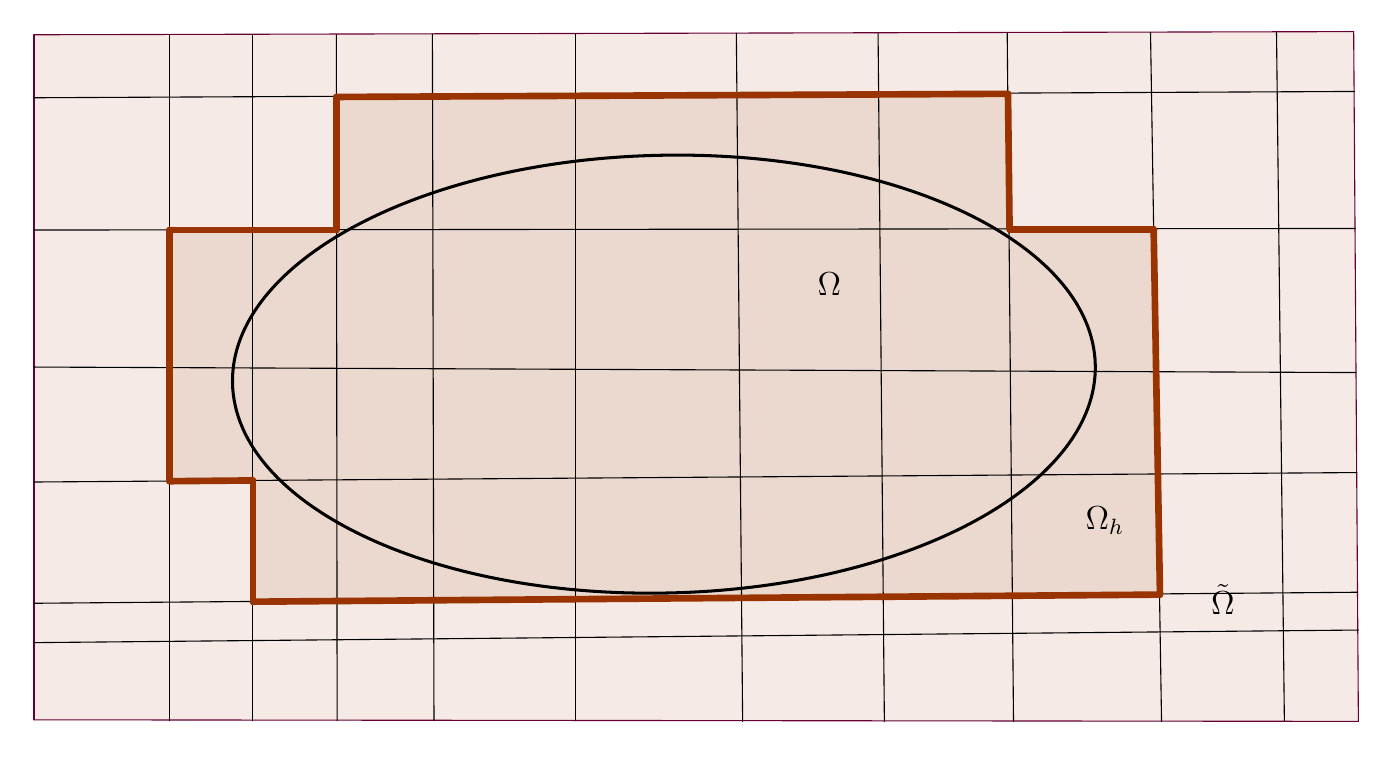
\begin{tikzpicture}[line cap=round,line join=round,>=triangle 45,x=1.0cm,y=1.0cm]
\clip(3.82,-7.67) rectangle (20.82,1.26);
\fill[color=zzttqq,fill=zzttqq,fill opacity=0.1] (3.9,1.17) -- (20.66,1.21) -- (20.72,-7.55) -- (3.9,-7.53) -- cycle;
\fill[line width=2.4pt,color=zzttqq,fill=zzttqq,fill opacity=0.1] (7.74,-1.31) -- (7.74,0.38) -- (16.27,0.42) -- (16.29,-1.3) -- (18.12,-1.3) -- (18.2,-5.94) -- (6.68,-6.03) -- (6.68,-4.49) -- (5.62,-4.5) -- (5.62,-1.31) -- cycle;
\draw [line width=1.1pt, rotate around={1.21:(11.9,-3.14)}] (11.9,-3.14) ellipse (5.48cm and 2.78cm);
\draw [color=wwqqtt] (3.9,1.17)-- (20.66,1.21);
\draw [color=wwqqtt] (20.66,1.21)-- (20.72,-7.55);
\draw [color=wwqqtt] (20.72,-7.55)-- (3.9,-7.53);
\draw [color=wwqqtt] (3.9,-7.53)-- (3.9,1.17);
\draw (3.9,0.37)-- (20.67,0.45);
\draw (20.68,-1.29)-- (3.9,-1.31);
\draw (3.9,-3.05)-- (20.69,-3.12);
\draw (20.7,-4.39)-- (3.9,-4.51);
\draw (3.9,-6.05)-- (20.71,-5.91);
\draw (3.9,-6.55)-- (20.72,-6.39);
\draw (5.62,1.17)-- (5.62,-7.54);
\draw (6.68,-7.54)-- (6.68,1.17);
\draw (7.74,1.17)-- (7.75,-7.54);
\draw (8.98,-7.54)-- (8.96,1.18);
\draw (10.78,1.18)-- (10.78,-7.54);
\draw (12.9,-7.55)-- (12.82,1.19);
\draw (14.62,1.19)-- (14.7,-7.55);
\draw (16.34,-7.55)-- (16.26,1.19);
\draw (18.08,1.2)-- (18.22,-7.55);
\draw (19.78,-7.55)-- (19.68,1.2);
\draw [line width=2.4pt,color=zzttqq] (7.74,-1.31)-- (7.74,0.38);
\draw [line width=2.4pt,color=zzttqq] (7.74,0.38)-- (16.27,0.42);
\draw [line width=2.4pt,color=zzttqq] (16.27,0.42)-- (16.29,-1.3);
\draw [line width=2.4pt,color=zzttqq] (16.29,-1.3)-- (18.12,-1.3);
\draw [line width=2.4pt,color=zzttqq] (18.12,-1.3)-- (18.2,-5.94);
\draw [line width=2.4pt,color=zzttqq] (18.2,-5.94)-- (6.68,-6.03);
\draw [line width=2.4pt,color=zzttqq] (6.68,-6.03)-- (6.68,-4.49);
\draw [line width=2.4pt,color=zzttqq] (6.68,-4.49)-- (5.62,-4.5);
\draw [line width=2.4pt,color=zzttqq] (5.62,-4.5)-- (5.62,-1.31);
\draw [line width=2.4pt,color=zzttqq] (5.62,-1.31)-- (7.74,-1.31);
\begin{scriptsize}
\draw (14,-2) node {\large{$\Omega$}};
\draw (17.5,-5) node{\large{$\Omega_h$}};
\draw (19,-6) node{\large{$\tilde{\Omega}$}};
\end{scriptsize}
\end{tikzpicture}
\caption{Définition des ensembles $\Omega$, $\tilde{\Omega}$ et $\Omega_h$ }
\label{fig2}
\end{figure}
\\
De plus, pour étudier la convergence de l'approximation, on suppose qu'il existe une famille d'opérateurs linéaires continus $(\tilde{\Pi}_h)_{h\in H}$ de $H^m(\Omega)$ dans $\tilde{V}_h$.

\end{document}
